
\section{变换坐标系}

通常，\PGFPlots{} 使用笛卡尔坐标。然而，人们可能希望在不同的坐标系中提供坐标。

在这种情况下，可以使用 |data cs| 键来标识输入坐标系：

\begin{pgfplotskey}{data cs=\mchoice{cart,polar,polarrad} (initially cart)}
    \label{key:data:cs}
    定义输入坐标的坐标系（`cs'）。如果参数与预期的坐标系不匹配，\PGFPlots{} 将应用变换。

    如果你的输入具有与坐标轴不同的坐标系，请使用 |data cs|。更准确地说，每种坐标轴类型都有自己的坐标系。例如，普通 |axis| 具有 |cart| 坐标系，而 |polaraxis| 具有 |polar| 坐标系。使用与坐标轴默认值不同的参数来使用 |data cs|，会指示 \PGFPlots{} 应用变换。

    在撰写本文时，\PGFPlots{} 支持以下 |data cs| 值：

    |data cs=|\declareandlabel{cart} 表示笛卡尔坐标系。它是通常 |axis|（或其对数变体）的坐标系。它可以有三个分量，$x$、$y$ 和 $z$。仅当你有非笛卡尔坐标轴时才需要指定它：
    %
% \usepgfplotslibrary{polar}
\begin{codeexample}[]
% requires \usepgfplotslibrary{polar}
\begin{tikzpicture}
\begin{polaraxis}
    \addplot coordinates {(90,1) (180,1)};
    \addplot+ [data cs=cart] coordinates {
        (1,0)
        (0.5,0.5)
    };
\end{polaraxis}
\end{tikzpicture}
\end{codeexample}

    |data cs=|\declareandlabel{polar} 是具有（角度，半径）的（二维）坐标系，即第一个分量“$x$”是角度，第二个分量“$y$”是半径。角度是周期范围 $[0,360)$ 中的数字；半径可以是任何数字。如果 |polar| 坐标有 $z$ 分量，则按原样取它（变换忽略它）。
    %
\begin{codeexample}[]
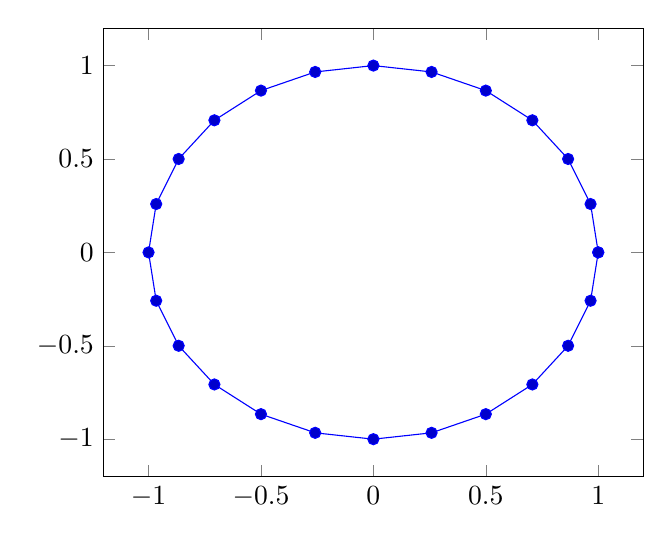
\begin{tikzpicture}
\begin{axis}
    \addplot+ [data cs=polar,domain=0:360] (\x,1);
\end{axis}
\end{tikzpicture}
\end{codeexample}

    |data cs|=\declareandlabel{polarrad} 类似于 |polar|，但它期望角度以弧度表示，即在周期范围 $[0,2\pi)$ 中。
    %
\begin{codeexample}[]
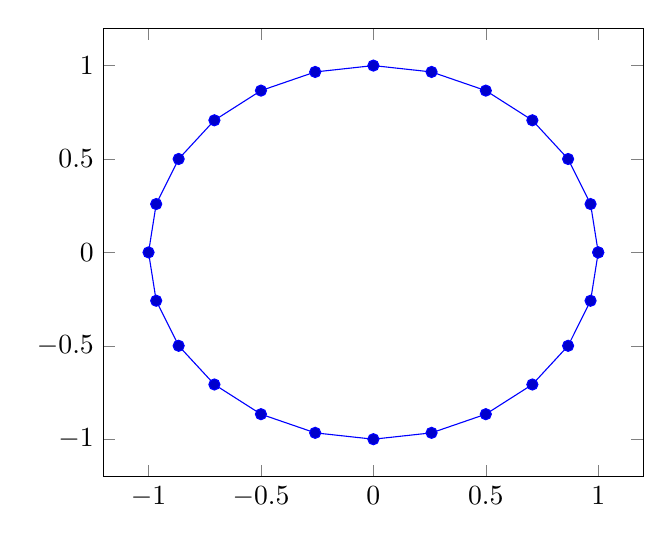
\begin{tikzpicture}
\begin{axis}
    \addplot+ [data cs=polarrad,domain=0:2*pi] (\x,1);
\end{axis}
\end{tikzpicture}
\end{codeexample}

    请注意，数学函数 |deg(|\meta{rad}|)| 将 \meta{rad} 转换为度，|rad(|\meta{degree}|)| 将 \meta{degree} 转换为弧度。因此，对于绘图表达式，|polar| 和 |polarrad| 或多或少等价。

\begin{codeexample}[]
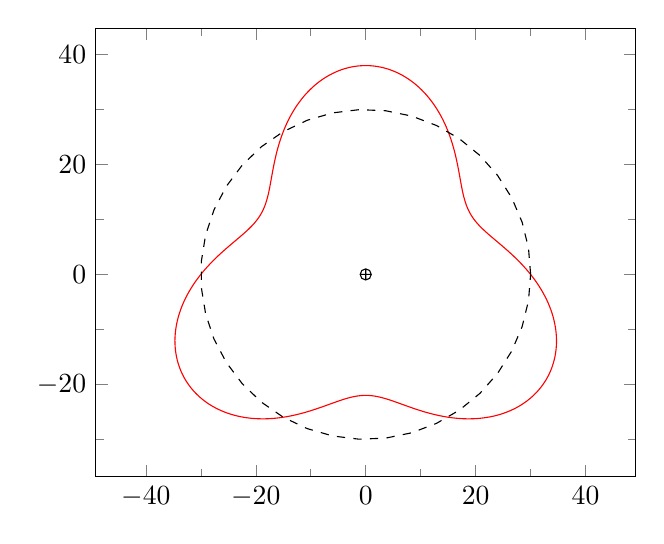
\begin{tikzpicture}
\begin{axis}[
    axis equal,
    minor tick num=1,
]
    \def\FREQUENCY{3}
\addplot [red,domain=0:360,samples=200,
    smooth,data cs=polar]
        (x,{30-8*sin(\FREQUENCY*x)});

\addplot [samples=40,domain=0:2*pi,dashed,
    data cs=polar] (deg(x),30);

\addplot [mark=oplus,only marks] coordinates {(0,0)};
 \end{axis}
\end{tikzpicture}
\end{codeexample}

    在撰写本文时，|data cs| 方法适用于大多数绘图处理器。但对于复杂的绘图处理器，可能需要尚不可用的进一步逻辑（例如，|quiver| 绘图处理器可能无法正确转换其方向向量）。\footnote{如果你遇到问题，请考虑编写错误报告或在 \TeX{} 在线讨论论坛中询问他人。}
\end{pgfplotskey}

\begin{command}{\pgfplotsaxistransformcs\marg{fromname}\marg{toname}}
    期望一组键中的当前点，以坐标系 \meta{fromname} 提供，并将它们替换为以 \meta{toname} 表示的相同坐标。

    输入时，坐标存储在 |/data point/x|、|/data point/y| 和 |/data point/z| 中（后者可以为空）。该宏将测试是否存在从 \meta{fromname} 到 \meta{toname} 的声明坐标变换并调用它。如果没有，它将尝试先转换为 |cart|，然后从 |cart| 转换为 \meta{toname}。如果那也不存在，则操作失败。
\end{command}

\begin{command}{\pgfplotsdefinecstransform\marg{fromname}\marg{toname}\marg{code}}
    定义一个新的坐标系变换。\meta{code} 应按 |\pgfplotsaxistransformcs| 所述获取输入并写入输出。

    实现新坐标系立即引发了应在何种数学模式下应用操作的问题。\PGFPlots{} 为通用操作以及每个单独坐标支持不同的所谓“坐标数学系统”。这些坐标数学系统可以使用基本 \PGF{} 数学运算、|fpu|，或者可能会出现 Lua\TeX{} 库。

    该系统的文档超出了本手册的范围。\footnote{即使没有 API 文档，它也相当全面，你肯定会同意……}如果你打算编写自己的变换，请考虑阅读源代码注释和现有变换的源代码。
\end{command}


\subsection{变换的相互作用}
\label{sec:transformation:interaction}

\PGFPlots{} 中有几个坐标映射。对于坐标流（|\addplot|）中遇到的每个坐标，它应用以下步骤：
%
\begin{enumerate}
    \item 在数学常量 |rawx|、|rawy|、|rawz| 中记住“原始”坐标，
        \index{rawx}\index{rawy}\index{rawz}%
    \item 应用 |pre filter|，\index{pre filter}
    \item 应用 |x coord trafo|（必要时取对数）和 |x filter|（按此顺序），
        \index{x coord trafo}%
    \item 应用 |y coord trafo|（必要时取对数）和 |y filter|，
        \index{y coord trafo}
    \item 应用 |z coord trafo|（必要时取对数）和 |z filter|，
        \index{z coord trafo}
    \item 应用 |filter point|，
        \index{filter point}%
    \item 从 |data cs| 变换到 |axis type| 的坐标系，
        \index{data cs}%
    \item 处理坐标堆叠（|stack plots=x| 和/或 |stack plots=y|）。
        \index{stack plots}%
\end{enumerate}
%
这里，|pre filter| 不接受参数；它只是准备以下过滤器。因此，第一个实际接受输入参数的项是 |x coord trafo|。此方法是解析的一部分；它接受“原始”坐标，该坐标可以是符号形式。|x coord trafo| 及其变体的输出是一个数字。此数字可以通过 |x filter| 及其变体进行过滤或变换。请注意，|x filter| 只接受一个参数：|x coord trafo| 的结果。

|x coord trafo| 的预期含义是定义用户提供的“原始”字符串形式如何进入 \PGFPlots{}。它也是唯一具有逆变换的变换，即键 |x coord inv trafo|。逆变换可用于从内部数字形式变换回最终用户的某个字符串。键 |x coord trafo| 只能定义为坐标轴的选项，即它不能提供给 |\addplot|。

|x filter| 及其变体的含义是变换数字或有条件地丢弃数字（从而丢弃整个坐标）。每个 |\addplot| 可以接收自己的（一组）过滤器。

键 |filter point| 接受\emph{所有}参数（更准确地说：前面步骤的结果）。它可以依赖于 $x$、$y$ 和 $z$，并且可以更改其中任何一个。它接受坐标的方式是通过键 |/data point/x|\index{/data point/x} 及其用于 $y$ 和 $z$ 的变体。原则上，|filter point| 是最通用的过滤器。然而，你可以同时定义 |x filter| 和 |filter point|，两者都会被应用。每个 |\addplot| 可以接收自己的 |filter point|。

键 |data cs| 的实现类似于 |filter point|，因为它接受所有先前映射步骤的结果。然而，它从明确定义的输入坐标系映射到某个明确定义的内部坐标系（这是坐标轴固有的）。每个 |\addplot| 可以接收自己的 |data cs|。

最后，|stack plots| 采取措施加/减结果。图的堆叠是坐标轴的一个属性；它不打算作为参数提供给 |\addplot|。\footnote{而且它似乎确实做了一些并非完全无用的事情。}
